% %%
\documentclass[atmosphere,article,accept,pdftex,moreauthors]{Definitions/mdpi}

% %%
% MDPI internal commands - do not modify
\firstpage{1}
\makeatletter
\setcounter{page}{\@firstpage}
\makeatother
\pubvolume{1}
\issuenum{1}
\articlenumber{0}
\pubyear{2024}
\copyrightyear{2024}
\externaleditor{Academic Editor: Firstname\linebreak Lastname}
\datereceived{2 January 2024}
\daterevised{17 January 2024} % Comment out if no revised date
\dateaccepted{29 January 2024}
\datepublished{ }
%\datecorrected{} % For corrected papers: "Corrected: XXX" date in the original paper.
%\dateretracted{} % For corrected papers: "Retracted: XXX" date in the original paper.
\hreflink{https://doi.org/} % If needed use \linebreak
%\doinum{}
%\pdfoutput=1 % Uncommented for upload to arXiv.org

% %%
% Full title of the paper (Capitalized)
\Title{Interannual Variation in Mainland China's Atmosphere Clearness Index Associated with El~Niño--Southern~Oscillation}

% MDPI internal command: Title for citation in the left column
\TitleCitation{Interannual Variation in Mainland China's Atmosphere Clearness Index Associated with El~Niño--Southern~Oscillation}

% Author Orchid ID: enter ID or remove command
\newcommand{\orcidauthorS}{0000-0002-1331-002X}
\newcommand{\orcidauthorZ}{0000-0001-7580-9128}
\newcommand{\orcidauthorW}{0000-0001-9239-9933}

% Authors, for the paper (add full first names)
\Author{Zongpeng Song $^{1}$\orcidS{}, Bo Wang $^{1}$, Hui Zheng $^{2,}$*\orcidZ{}, Shu Wang $^{1}$\orcidW{}, Xiaolin Liu $^{1}$ and Shuanglong Jin $^{1}$}

%\longauthorlist{yes}

% MDPI internal command: Authors, for metadata in PDF
\AuthorNames{Zongpeng Song, Bo Wang, Hui Zheng, Shu Wang, Xiaolin Liu and Shuanglong Jin}

% MDPI internal command: Authors, for citation in the left column
\AuthorCitation{Song, Z.; Wang, B.; \linebreak Zheng, H.; Wang, S.; Liu, X.; Jin, S.}

% Affiliations / Addresses (Add [1] after \address if there is only one affiliation.)
\address{%
$^{1}$ \quad National Key Laboratory of Renewable Energy Grid-Integration, China Electric Power Research Institute, Beijing 100192, China; songzongpeng@epri.sgcc.com.cn (Z.S.); wangbo@epri.sgcc.com.cn (B.W.); wangshu@epri.sgcc.com.cn (S.W.); liuxiaolin@epri.sgcc.com.cn (X.L.); jinshuanglong@epri.sgcc.com.cn (S.J.)\\
$^{2}$ \quad Laboratory of Regional Climate-Environment Research for Temperate East Asia, Institute of Atmospheric Physics, Chinese Academy of Sciences, Beijing 100029, China; hzheng\_iap@outlook.com (H.Z.) }

% Contact information of the corresponding author
\corres{Correspondence: hzheng\_iap@outlook.com}

%\simplesumm{} % Simple summary

% Abstract (Do not insert blank lines, i.e., \\)
\abstract{Atmosphere clearness is the single most essential parameter determining surface solar radiation. However, few studies have investigated the interannual variations in China's atmosphere clearness and the impacts of El~Niño--Southern~Oscillation on it. This study aims to fill the knowledge gap by calculating the clearness index using the China Meteorological Forcing Dataset version 1.7 and then analyzing the correlations between the interannual anomaly and the Niño-3.4 index. The results show that there is a significantly negative correlation in the southeastern coastal regions, northern Xinjiang, northeastern Xizang, and areas from northern Hebei to middle Inner Mongolia. In these areas, the higher the ENSO index, the lower the clearness index, and, coincidingly, positive precipitation anomalies are reported in previous studies. The impacts of El~Niño and La~Niña vary with seasons. The ENSO events have generally opposite impacts in the seasons other than summer. El~Niño tends to decrease the clearness index, while La~Niña tends to decrease the atmosphere clearness in most territories of China. The impacts are different in the places of statistical significance. The negative impacts of El~Niño are significant in the southeastern coastal regions of China in winter and in northeast China in autumn. The positive impacts of La~Niña are significant in the southwestern and northeastern China in the autumn. In these seasons, ENSO's impacts scale with the strength of the event. Stronger events amplify the magnitude of the anomalies, while the spatial patterns of the anomalies are kept almost invariant. In summer, ENSO's impacts exhibit different characteristics than in the other seasons and between the El~Niño and La~Niña events. For the El~Niño events, the impacts are insignificant in most territories of China, even for the strong ones. La~Niña has a larger influence on the summertime clearness than El~Niña, and the spatial pattern of the La~Niña's impacts varies with the event strength. The anomalies during strong La~Niña events have a tripolar pattern with a positive anomaly in south and north China and a negative anomaly in between. The pattern suggests that the relationship between the clearness index and precipitation is different during strong La~Niña events. These findings would provide valuable insights into the interannual variations of atmosphere clearness in China and could be clues to further investigation. The revealed impacts of El~Niño--Southern~Oscillation should be important for developing solar energy.}

% Keywords
\keyword{El~Niño--Southern~Oscillation; solar radiation; atmosphere clearness; interannual variation; China}

% %%
\begin{document}

\section{Introduction}\label{sec:introduction}

El~Niño--Southern~Oscillation (ENSO) is a recurring climate pattern across the tropical Pacific. The phenomenon involves the interaction between the ocean and the atmosphere~\cite{bjerknes1969MWR}. The Pacific Ocean's surface temperature swings between relatively warm and cold phases, producing events called El~Niño and La~Niña, respectively~\cite{philander1989}. The swing in ocean states is coupled with the overlaying atmosphere. The variation in the atmospheric pressure difference between Australia and Indonesia and that of the eastern South Pacific is called Southern~Oscillation~\cite{walker1928MWR, julian1978MWR}. ENSO follows irregular periods of two to seven years~\cite{latif1998JGRO,rasmusson1982MWR}, bringing predictable shifts in ocean surface temperature~\cite{lin2019SR} and disrupting the \mbox{wind~\cite{rasmusson1982MWR, hu2023CD, maruyama1988JMSJ, kane2004IJC,wallace1998JGRO}} and convection~\cite{yang2013JAS} patterns across the tropics. These changes have a cascade of global-scale climatic impacts~\cite{trenberth1998JGRO, annamalai2023JC, yeh2018RG}.

Extensive studies have shown that ENSO profoundly impacts China's climate system~\cite{huang1989AAS, wu2009JC, chen2012CJOL}, including precipitation, temperature, and aerosol concentration. There is a tripolar anomaly pattern in the summer precipitation (i.e., June, July, and August) during the El~Niño decaying year, with a positive anomaly in south and north China and a negative anomaly in between~\cite{huang1989AAS, huang2012AAS}. During the El~Niño developing year, the anomaly of the tripolar pattern is reversed~\cite{duan2023JC}. The summertime precipitation anomaly pattern is different from other seasons. Excessive (deficient) precipitation in winter, spring, and autumn tends to occur in southern China during the El~Niño developing (decaying) year~\cite{zhang1999AAS}. The impact of ENSO on temperature is significant in northeast China, and the impact differs before and after the mid-1970s. Before the mid-1970s, the northeast China summer was warmer than normal during the El~Niño developing years and colder during the La~Niña developing years, whereas the opposite anomalies occurred after the mid-1970s~\cite{wu2010JGRA}. ENSO impacts aerosol concentrations in eastern China, but the impacts are complex. During a Central Pacific El~Niño event from 1994 to 1995, the aerosol concentration increased during the mature phases of the event while decreasing in the decaying phases~\cite{feng2016JGRA}. The variation in aerosol concentration differs among the La~Niña events~\cite{feng2017JGRA}. During the mature phase of a strong event from 1998 to 1999, the spatial pattern of the aerosol concentration showed a dipole pattern, with a relative high in South China and a relative low in North China. The dipole distribution is reversed in a moderate event from 2000 to 2001~\cite{feng2017JGRA}. Based on more extended datasets from 1980 to 2016, it is found that El~Niño events can promote the accumulation of aerosols in most areas of eastern China, whereas La~Niña events lower aerosol concentration in most areas except the middle Yangtze River and Yellow \mbox{River basins~\cite{sun2018JGRA}}.

However, few studies have investigated the impacts of ENSO on China's atmosphere clearness. Atmosphere clearness is the single most essential parameter determining surface solar radiation. It measures the transparency of the Earth's atmosphere to solar radiation~\mbox{\cite{liu1960SE, udo2000SE}}. Surface solar radiation is the product of atmosphere clearness and extraterrestrial solar radiation~\cite{jung2016A, apeh2021S, olukemisoneye2021A}. Extraterrestrial solar radiation is deterministic as a function of astronomical geometry~\cite{liu1960SE, cooper1969SE}, whereas atmosphere clearness is variate and dominates the variation of surface \mbox{solar radiation~\cite{apeh2021S, udo2000SE}}. The variations in the atmosphere's clearness are driven by various parameters that affect the absorption and scattering of solar radiation both directly and indirectly~\cite{che2005GRL, liu1960SE}. The directly influential parameters include cloud amount, water vapor content, and aerosol concentration~\cite{tang2016ACP}, whereas indirect parameters include wind speed~\cite{zhao2022JC, sun2018JGRA}. As ENSO has significant impacts on these parameters, the impacts are expected to be reflected in the atmosphere's clearness.

This study aims to fill the knowledge gap by analyzing the interannual variation of China's atmosphere clearness and by revealing its linkage with ENSO\@. In the practice of solar energy forecasting and planning, atmosphere clearness is widely used, as it could be the only piece of information needed to characterize the status of the atmosphere~\cite{perez1990SE, lauret2022S}. The revealed impacts of ENSO would provide valuable insights into the interannual variations of atmosphere clearness in China and are informative for various solar energy applications.

The paper is organized as follows. Section~\ref{sec:datamethods} describes the used data, the calculation of the clearness index, and the analysis method. Section~\ref{sec:results} provides the results and discussion. Finally, Section~\ref{sec:conclusions} draws conclusions.

% %%
\section{Data and Methods}\label{sec:datamethods}

\subsection{Clearness Index}\label{sec:clearnessindex}

The clearness index is a measure of atmosphere clearness in terms of solar radiation. The index is defined as the ratio of the global horizontal radiation to the extraterrestrial radiation. Its value varies from 0 to 1. The higher the value, the clearer the sky.

Global horizontal radiation is the total solar radiation received by a horizontal surface. We used the 3-hourly global horizontal irradiance data from the China Meteorological Forcing Dataset (CMFD) version 1.7. The CMFD global horizontal irradiance is derived based on the European Centre for Medium-Range Weather Forecasts (ECMWF) ERA5 reanalysis data~\cite{hersbach2020QJRMS}. In-situ observation data from the China Meteorological Administration and NOAA National Centers for Environmental Information are used to correct the biases in ERA5~\cite{he2020SD}.

The clearness index is calculated at each 0.1\textdegree{} CMFD grid cell. CMFD v1.7 spans from 1950 to 2020. We used the period from December 1983 to November 2020, during which in-situ observations used in the bias correction are more reliable. The clearness index is calculated at each 3-hourly CMFD time step. Only the daytime values are considered, ensuring the stability of the calculation. In this study, we define the daytime period as the extraterrestrial solar radiation being greater than 120~\(\mathrm{W\,m^{-2}}\) \texttimes 3~h, which is equivalent to a solar azimuth angle of approximately 85\textdegree{}.

\subsection{Extraterrestrial Solar Radiation}\label{sec:extraterrestrial}

Extraterrestrial radiation is the radiation that would reach the surface if there were no atmospheric effects. We calculated the 3-hourly extraterrestrial solar radiation, \(H_0\), using the following equations~\cite{udo2000SE}:
\begin{linenomath}
  \begin{equation}\label{eq:esr}
    H_0 = \frac{12}{\pi} I_{sc} E_0 \left[\sin\delta \sin\phi(\omega_2 - \omega_1) + \cos\delta \cos\phi(\sin\omega_2-\sin\omega_1)\right] \text{,}
  \end{equation}
\end{linenomath}
where \(I_{sc} = 1367\,\mathrm{W\,m^{-2}}\times{}3600\,\mathrm{s} = 4921.2\,\mathrm{KJ\,m^{-2}\,h^{-1}}\) is the solar constant. \(E_0\) is the eccentricity correction factor of the Earth's orbit. It is calculated as~\cite{udo2000SE}:
\begin{linenomath}
  \begin{multline}\label{eq:eccentricity}
    E_0 = 1.000110
    + 0.034221\cos\gamma
    + 0.001280\sin\gamma \\
    + 0.000719\cos(2\gamma)
    + 0.000077\sin(2\gamma) \text{.}
  \end{multline}
\end{linenomath}

\(\gamma\) is the fractional year in radians.
\begin{linenomath}
  \begin{equation}\label{eq:fractionalyear}
    \gamma = \frac{2\pi}{365}(d_n - 1) \text{,}
  \end{equation}
\end{linenomath}
where \(d_n\) is the number of days since January 1st 00Z. For leap years, the denominator is 366 instead of 365. \(\delta \in [-23.45^\circ, 23.45^\circ]\) is the solar declination, which is calculated as follows~\cite{udo2000SE}:
\begin{linenomath}
  \begin{multline}\label{eq:declination}
    \delta = 0.006918
    - 0.399912\cos\gamma
    + 0.070257\sin\gamma
    - 0.006758\cos(2\gamma)
    + 0.000907\sin(2\gamma) \\
    - 0.002697\cos(3\gamma)
    + 0.00148\sin(3\gamma) \text{.}
  \end{multline}
\end{linenomath}
\(\omega_1\) and \(\omega_2\) are the solar hour angles at the beginning and the end of the 3 h, respectively. The solar hour angle (\(\omega\)) is calculated following the NOAA global monitoring division (\url{https://gml.noaa.gov/grad/solcalc/solareqns.PDF} accessed on 27 December 2023):
\begin{linenomath}
  \begin{equation}\label{eq:hourangle}
    \omega = \frac{\pi}{12}\left(t - 12 + t_{eq}\right)\text{,}
  \end{equation}
\end{linenomath}
where \(t\) is the local time in hours. \(t_{eq}\) is the equation of time in hours.
\begin{linenomath}
  \begin{multline}\label{eq:equationoftime}
    t_{eq} = \frac{229.18}{60}[0.000075
      + 0.001868\cos\gamma
      - 0.32077\sin\gamma \\
      - 0.014616\cos(2\gamma)
      - 0.040849\sin(2\gamma)] \text{.}
  \end{multline}
\end{linenomath}

\subsection{El~Niño--Southern~Oscillation Index}\label{sec:enso}

We used the Niño-3.4 index to characterize the ENSO cycles. The Niño-3.4 index is defined as the sea surface temperature anomaly (SSTA) averaged over the region of 5~\textdegree{}N--5~\textdegree{}S, 170~\textdegree{}--120~\textdegree{}W. The month values of the index are available from the National Oceanic and Atmospheric Administration website (\url{https://psl.noaa.gov/data/correlation/nina34.anom.data} accessed on 30 December 2023).

We used the El~Niño and La~Niña events defined by the NOAA Climate Prediction Center (\url{https://www.cpc.ncep.noaa.gov/products/analysis_monitoring/ensostuff/ONI_v5.php} accessed on 30 December 2023). The El~Niño and La~Niña events are defined if the three-month running mean of the Niño-3.4 index is 0.5~\textdegree{}C above and \textminus{}0.5~\textdegree{}C below the long-term average by a minimum of five consecutive overlapping seasons, respectively~\cite{kousky2007WF}. During the period from December 1983 to November 2020, there were a total of ten El~Niño events and eight La~Niña events. The El~Niño events occurred in 1986--1987, 1987--1988, 1991--1992, 1994--1995, 1997--1998, 2002--2003, 2004--2005, 2006--2007, 2009--2010, 2014--2015, 2015--2016, and 2018--2019. The La~Niña events occurred in 1983--1984, 1984--1985, 1988--1989, 1995--1996, 1998--1999, 1999--2000, 2000--2001, 2005--2006, 2007--2008, 2008--2009, 2010--2011, 2011--2012, 2016--2017, and 2017--2018. These events mature in the boreal winter (December--February) and decay from the following spring (March--May).

\subsection{Analysis Methods}\label{sec:stats}

We calculated the monthly clearness index by arithmetically averaging the 3-hourly values. The arithmetic average rather than the average weighted by the extraterrestrial solar radiation would better reveal the dynamics of the atmosphere. Then, the interannual anomalies of the clearness index were calculated by subtracting the long-term monthly mean from the monthly values and are used in the following analyses.

The analyses consist of two parts. The first part examined the spatial distribution and temporal variability of the clearness index in China. The second part revealed the impacts of ENSO on the clearness index. The impacts were revealed with two approaches. First, we calculated the parametric Pearson and nonparametric Spearman correlation coefficient between the monthly anomalies in the clearness index and Niño-3.4 index. Second, we analyzed the difference in the clearness index between the El~Niño and La~Niña events versus the long-term mean. The statistical significance of both the correlation coefficient and the difference were tested. The significance level is set to 0.1, considering the weak signal of the ENSO's impacts.

% %%
\section{Results and Discussion}\label{sec:results}

\subsection{Spatial Distribution and Temporal Variations of the Clearness Index}\label{sec:clearnessindexpattern}

Figure~\ref{fig:distribution} shows the spatial distribution of the 37-year averaged (December 1983 to November 2020) clearness index in China. The average value is 0.51. The atmosphere clearness is higher in the northern and western regions and lower in the southern and eastern regions. The highest atmosphere clearness occurs in the western Xizang, with a value of 0.66 (the 0.99 quantile). The high clarity over the area is attributable to the thin atmosphere~\cite{duan2012AAS} and dry climate~\cite{wang2018IJCa}. The clearness index is the lowest in the border areas among Sichuan, Chongqing, and Guizhou, with a value of 0.03 (the 0.01 quantile). The area is downstream of the Tibetan Plateau and abundant with water vapor, clouds, and precipitation.

\begin{figure}[H]
  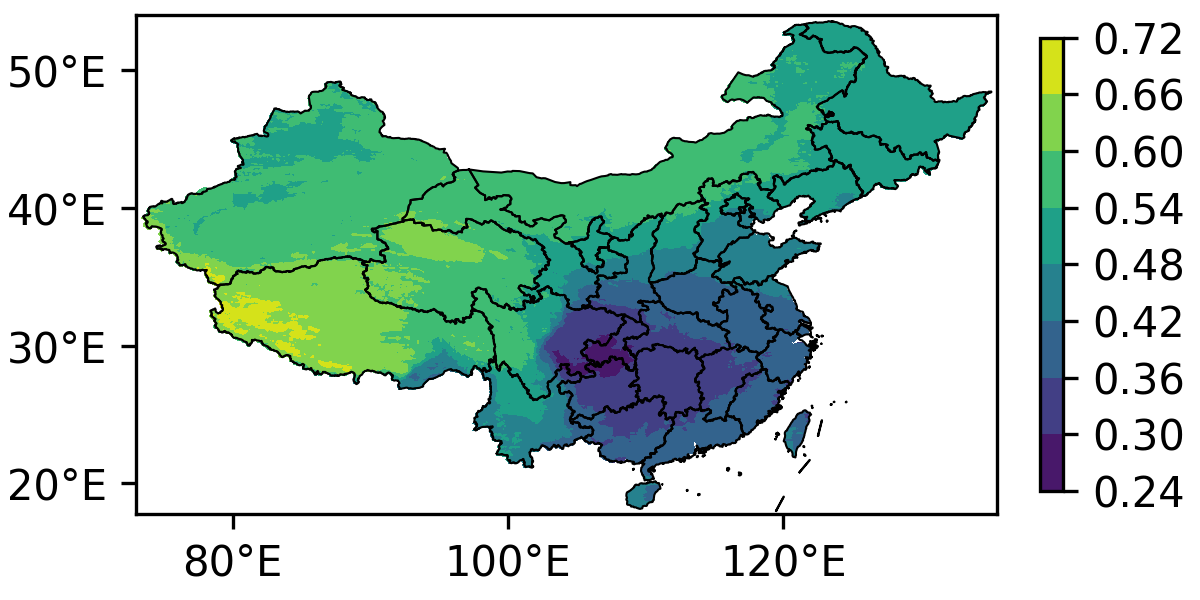
\includegraphics[width=0.8\textwidth]{fig/distribution.png}
  \caption{Spatial distribution of the multi-year averaged clearness index from December 1983 to November 2020. \label{fig:distribution}}
\end{figure}

The seasonal variation in the clearness index is notable in most territories of China, as shown in Figure~\ref{fig:season}. The phases of the variation in northwest and southeast China are different, hinting at a distinction in the controlling atmospheric dynamics. In the Northwest, the clearness index is higher in autumn and winter and lower in spring and summer. The region is far from a water source. Midlatitude westerly is the primary external source of water vapor~\cite{yang2008JAMS, zhang2021FES}, and the precipitation is concentrated in the summer~\cite{chen2012JC}. A relatively abundant water vapor and precipitation lower the clearness index in the summer, whereas a relatively dry climate in winter improves the atmosphere's clearness. In the Southeast, the variation is the opposite. The clearness index is higher in summer and lower in the winter. In cold seasons, the area has ample water vapor and clouds. The water vapor is brought by the wintertime southern branch of the subtropical westerly around the Tibetan Plateau~\cite{yeh1950T, ding2017JGRA, li2015AASa, yin2023FES}. The water vapor interplays with the cold air from the north and is condensed into clouds. This interaction results in one of the most substantial and frequent wintertime stratus clouds in the world~\cite{klein1993JC, jin2009JGRA, chen2022AOSL}, which lowers the clearness index.

\begin{figure}[H]
  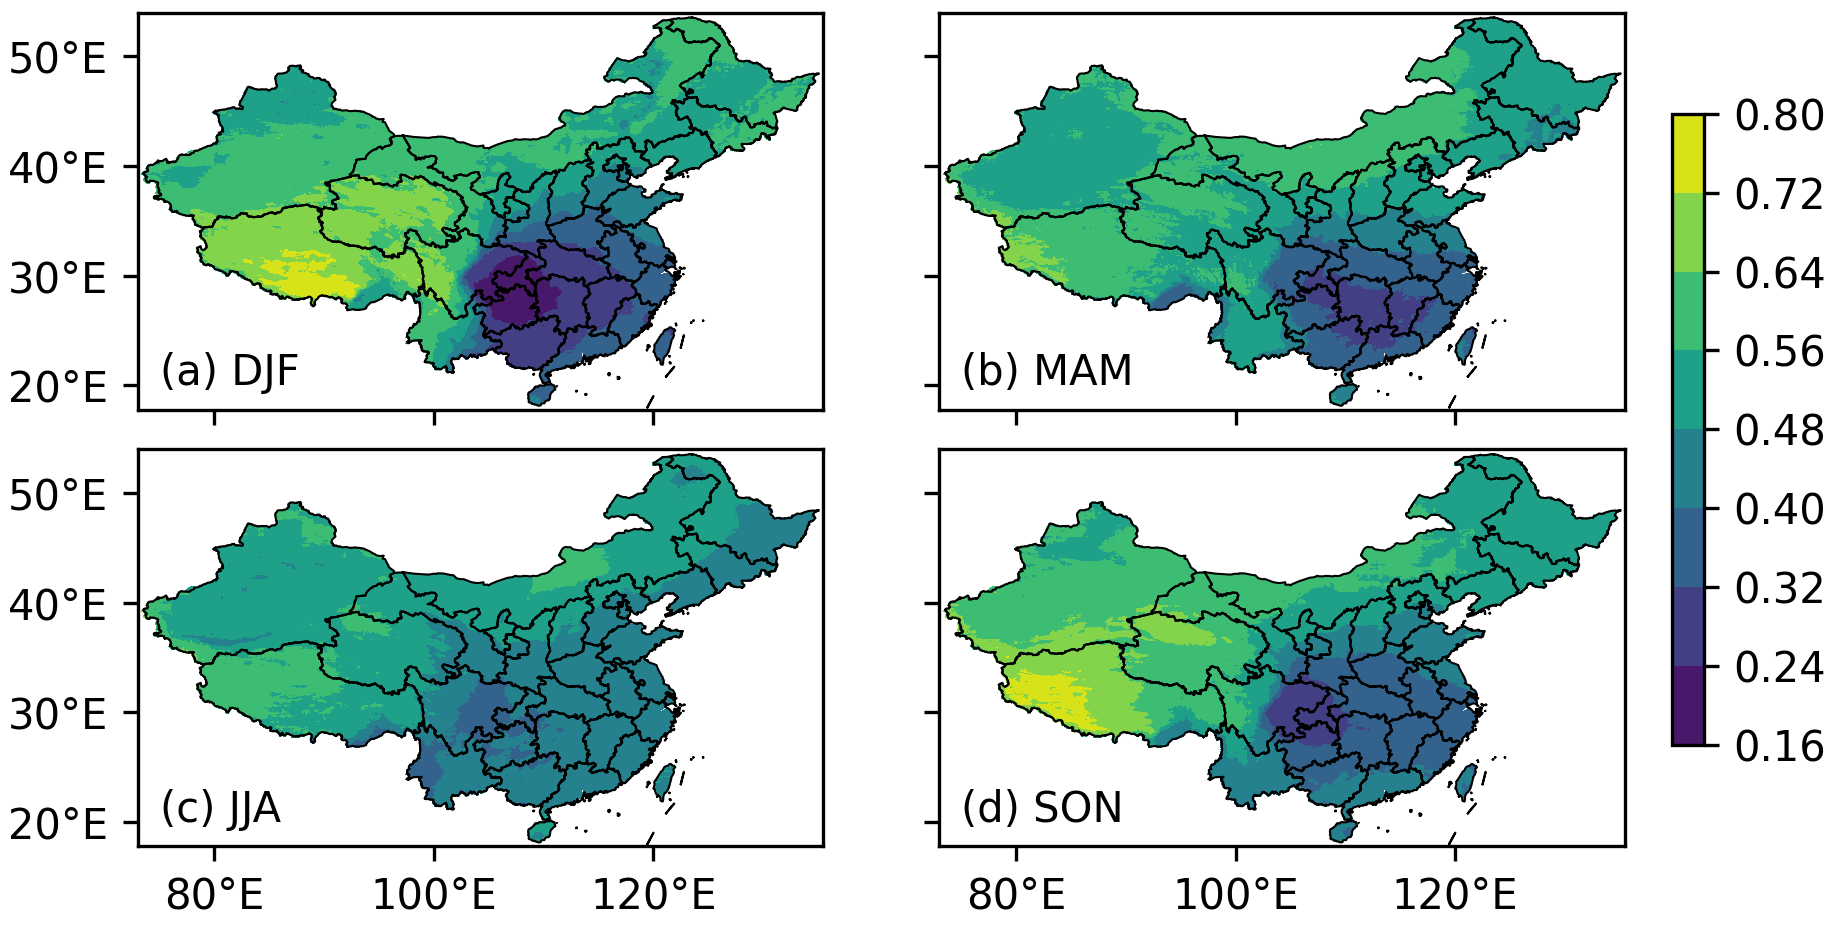
\includegraphics[width=14cm]{fig/seasons.png}
  \caption{Seasonal distribution of the multi-year averaged clearness index from December 1983 to November 2020. (\textbf{a}) DJF for December, November, and January. (\textbf{b}) MAM for March, April, and May. (\textbf{c}) JJA for June, July, and August. (\textbf{d}) SON for September, October, and November. \label{fig:season}}
\end{figure}


Figures~\ref{fig:szv} and \ref{fig:iav} intercompare the seasonal and interannual variabilities in the clearness index. For fair intercomparisons, the variabilities are normalized by the multi-year averaged climatology. The normalized variability is also referred to in the literature as the coefficient of variability. In most territories of China, the seasonal variability is overwhelming in magnitude over the interannual variability. The coefficient of seasonal variability is 0.11 on average. It is more significant in the areas from the southern Tibetan Plateau to western Yunnan, northeastern China, and eastern Sichuan Basin than in the other regions of China. The seasonal variation of the Indian monsoon~\cite{hrudya2021MAP}, Northeast cold vortex~\cite{wu2021ESS}, and East Asian monsoon~\cite{ding2005MAP} play a role in these three regions, respectively. The interannual variability has a similar spatial distribution to the seasonal variability. However, its magnitude varies with seasons. The average coefficient of interannual variability is 0.082, 0.065, 0.061, and 0.067 for winter, spring, summer, and autumn, respectively. Winter has the largest variability, as shown in Figure~\ref{fig:iav}a. It is interesting to notice that topography plays an important role. The phenomenon is evident in the Tianshan, Qilian, and Xing'an Mountains in autumn and winter; however, the reason is unclear and needs further investigation.

\begin{figure}[H]
  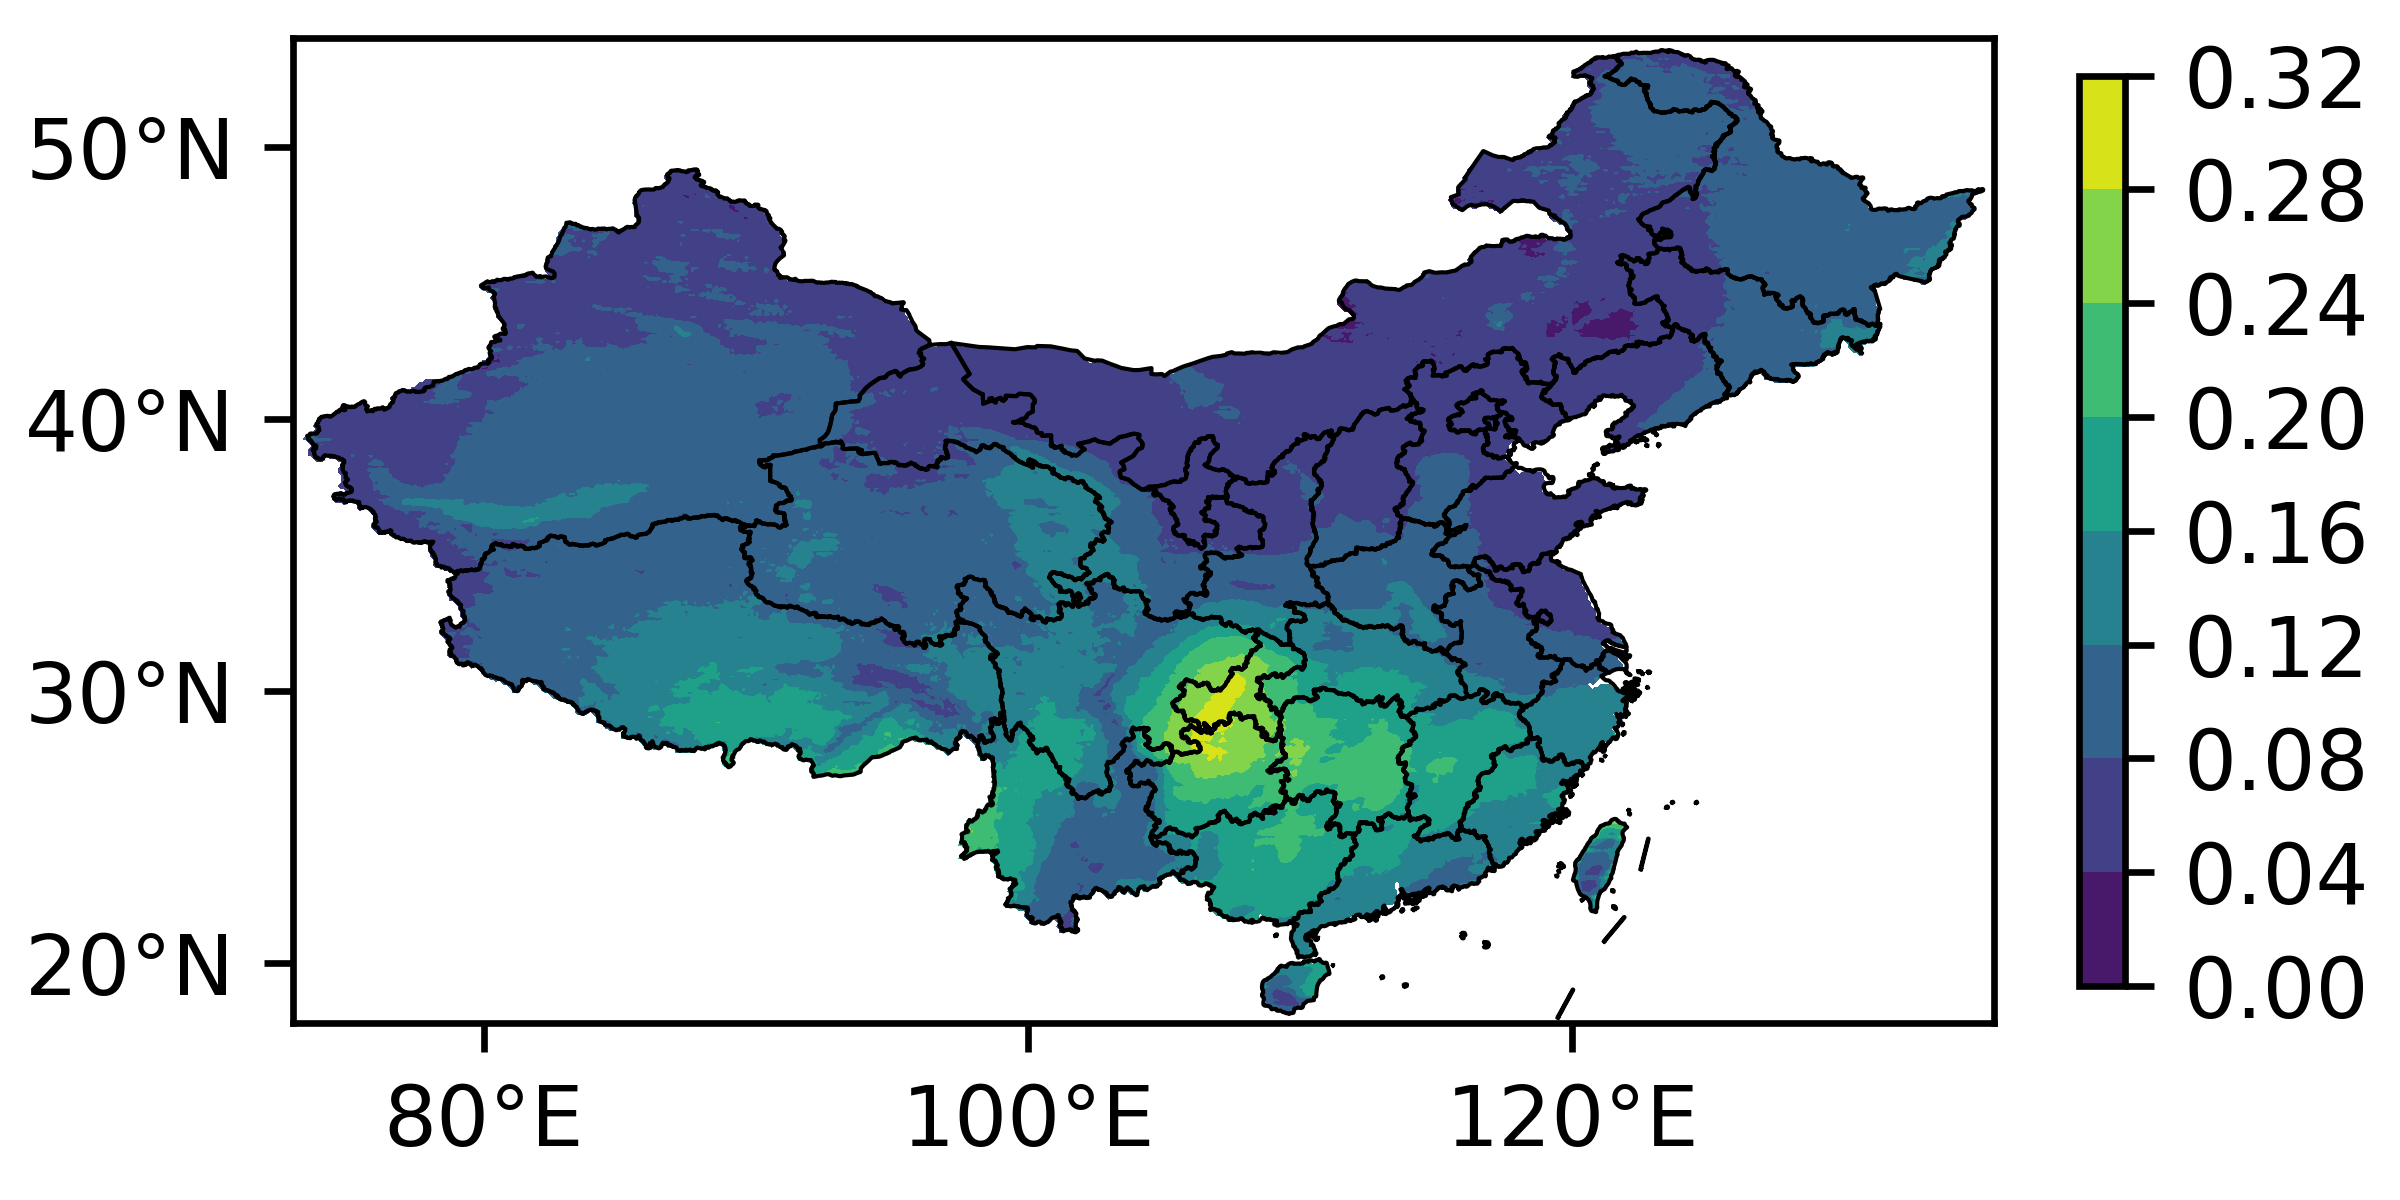
\includegraphics[width=10.16cm]{fig/szv.png}
  \caption{Coefficient of seasonal variability in the clearness index. The coefficient is defined as the ratio of standard deviation to the multi-year average. The variability is measured by the standard deviation of the multi-year averaged monthly clearness index. The multi-year average is calculated from December 1983 to November 2020. \label{fig:szv}}
\end{figure}

\begin{figure}[H]
  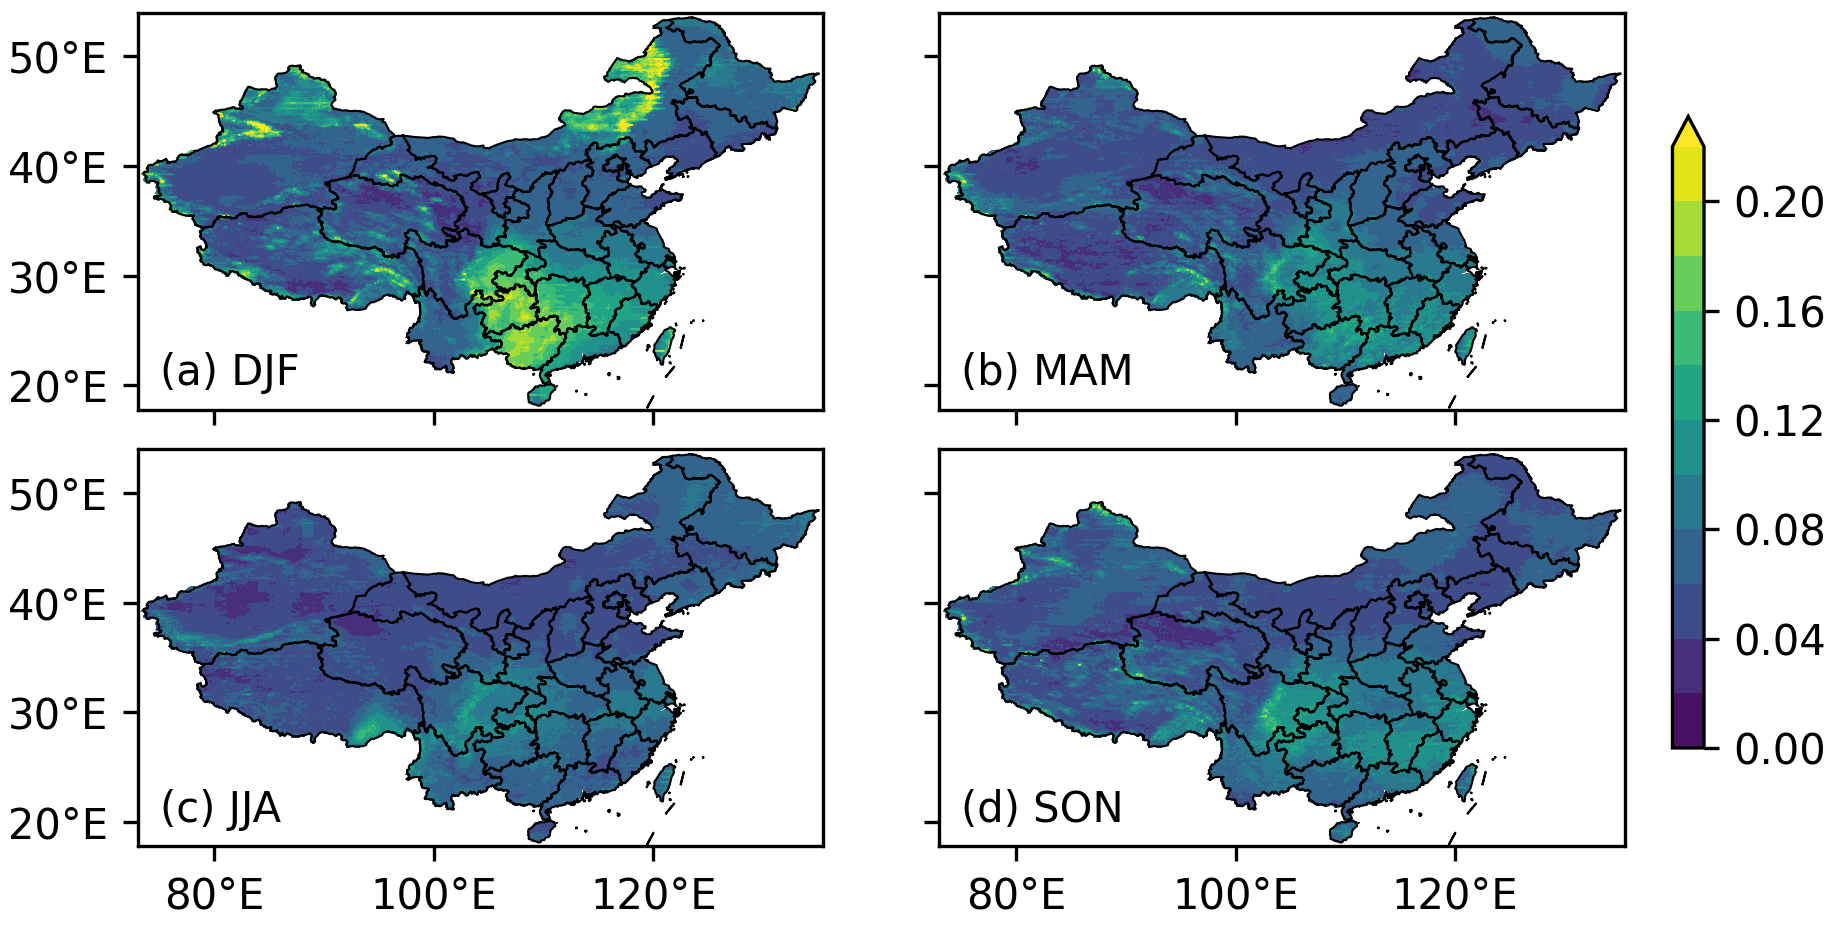
\includegraphics[width=14cm]{fig/iav.png}
  \caption{Same as in Figure~\ref{fig:szv}, but for the interannual variability in the four seasons. \label{fig:iav}}
\end{figure}

\subsection{Impacts of the El~Niño and La~Niña Events on the Clearness Index}\label{sec:clearnessindexanomalies}

Figure~\ref{fig:correlation} shows the correlation coefficient between the monthly clearness index and the simultaneous Niño-3.4 index. The two types of correlation coefficients (i.e., the parametric Pearson and nonparametric Spearman correlation coefficients) exhibit a similar spatial pattern. There is a significantly negative correlation in the southeast coastal regions of China, the northeastern Xizang, northern Xinjiang, and northern Heibei to middle Inner Mongolia, whereas the correlation is significantly positive in eastern Yunnan and eastern Inner Mongolia. The negative correlation in the southeast coastal regions is consistent with previous studies of regional wetness~\cite{wang2017IJC}: the El~Niño events increase the westness and promote precipitation there. In the areas from northern Hebei to middle Inner Mongolia, the El~Niño events have been shown to be capable of generating anticyclonic anomalies in the Northeast. The associated southerly anomalies could reduce wind speed and increase low-level atmospheric humidity in winter~\cite{zhao2022JC}. The lowered wind speed and elevated humidity would in consequence reduce atmosphere clearness. The positive correlation in eastern Inner Mongolia would be another consequence of the Northeast anticyclonic anomalies. The hypothesis needs further examination, but it is beyond the scope of this paper. Despite the broad understanding that ENSO has no direct impact on northwestern China, we found a significantly negative correlation in northern Xinjiang. This finding is in line with previous studies of precipitation~\cite{lu2019ASL}. One possible mechanism is that El~Niño would warm the Indian Ocean. The warmer Indian Ocean extends the South Asia high towards the south. The cyclonic anomalies associated with the extension could bring water vapor from the Indian Ocean, through the Iranian Plateau, and into northern Xinjiang~\cite{lu2019ASL}. The increased water vapor elevates clouds and precipitation and decreases \mbox{the clearness index}.

\begin{figure}[H]
  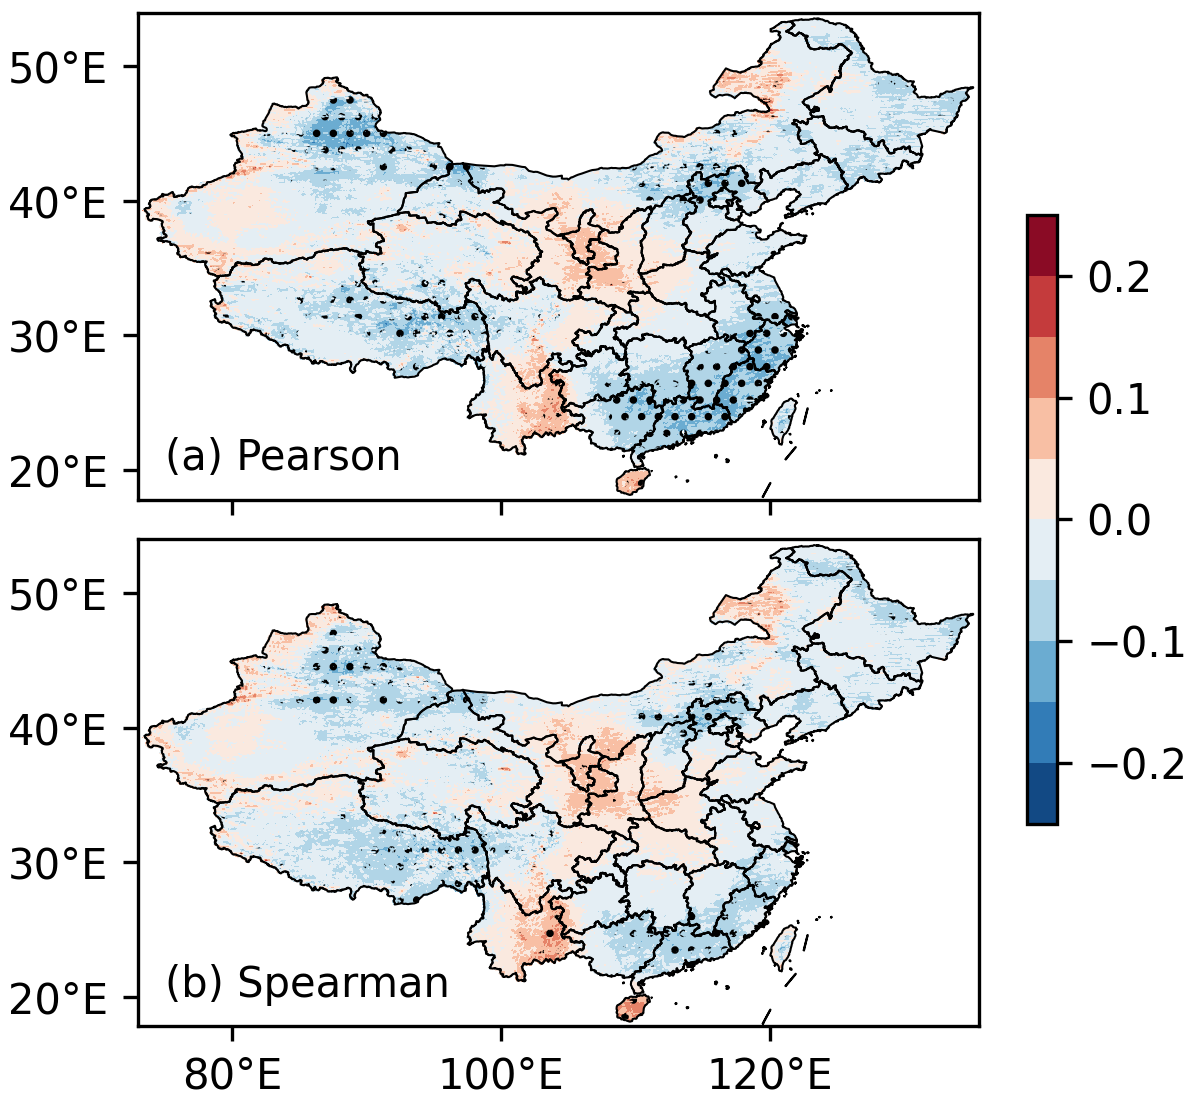
\includegraphics[width=10.16cm]{fig/correlation.png}
  \caption{Correlation between the clearness index and the Niño-3.4 index. (\textbf{a}) Pearson's correlation coefficient, and (\textbf{b}) Spearman's correlation coefficient. Black dots denote the areas with a significance level of 0.1. \label{fig:correlation}}
\end{figure}

Figure~\ref{fig:elnino} shows the anomalies in the clearness index averaged over all the El~Niño events (i.e., Figure~\ref{fig:distribution}). Unlike the precipitation anomaly patterns~\cite{huang1989AAS, zhang1999AAS, huang2012AAS}, the anomalies in the clearness index are statistically significant in particular areas and seasons. Significantly negative correlations occur in the southeastern coastal regions of China in winter and southern northeast China in autumn. The areas are consistent with previous studies on precipitation anomalies. The negative anomalies in the clearness index coincide with the positive anomalies of the winter precipitation in the southeastern coastal regions~\cite{wang2017IJC} and the autumn precipitation in northeast China~\cite{gu2022ACCR}. The positive anomalies in the clearness index are consistent with the negative precipitation anomalies found in spring and eastern Yunnan~\cite{li2021CDb}. However, it is interesting to notice that there is no significant correlation in summer. The pattern is different from that of precipitation~\cite{huang1989AAS, huang2012AAS, zhang1999AAS}. The distinction suggests different mechanisms of the summertime clearness index and precipitation. The difference may be due to the changes in wind. However, the investigation of the phenomenon and the underlying mechanism is lacking in the literature and needs further study.

\begin{figure}[H]
    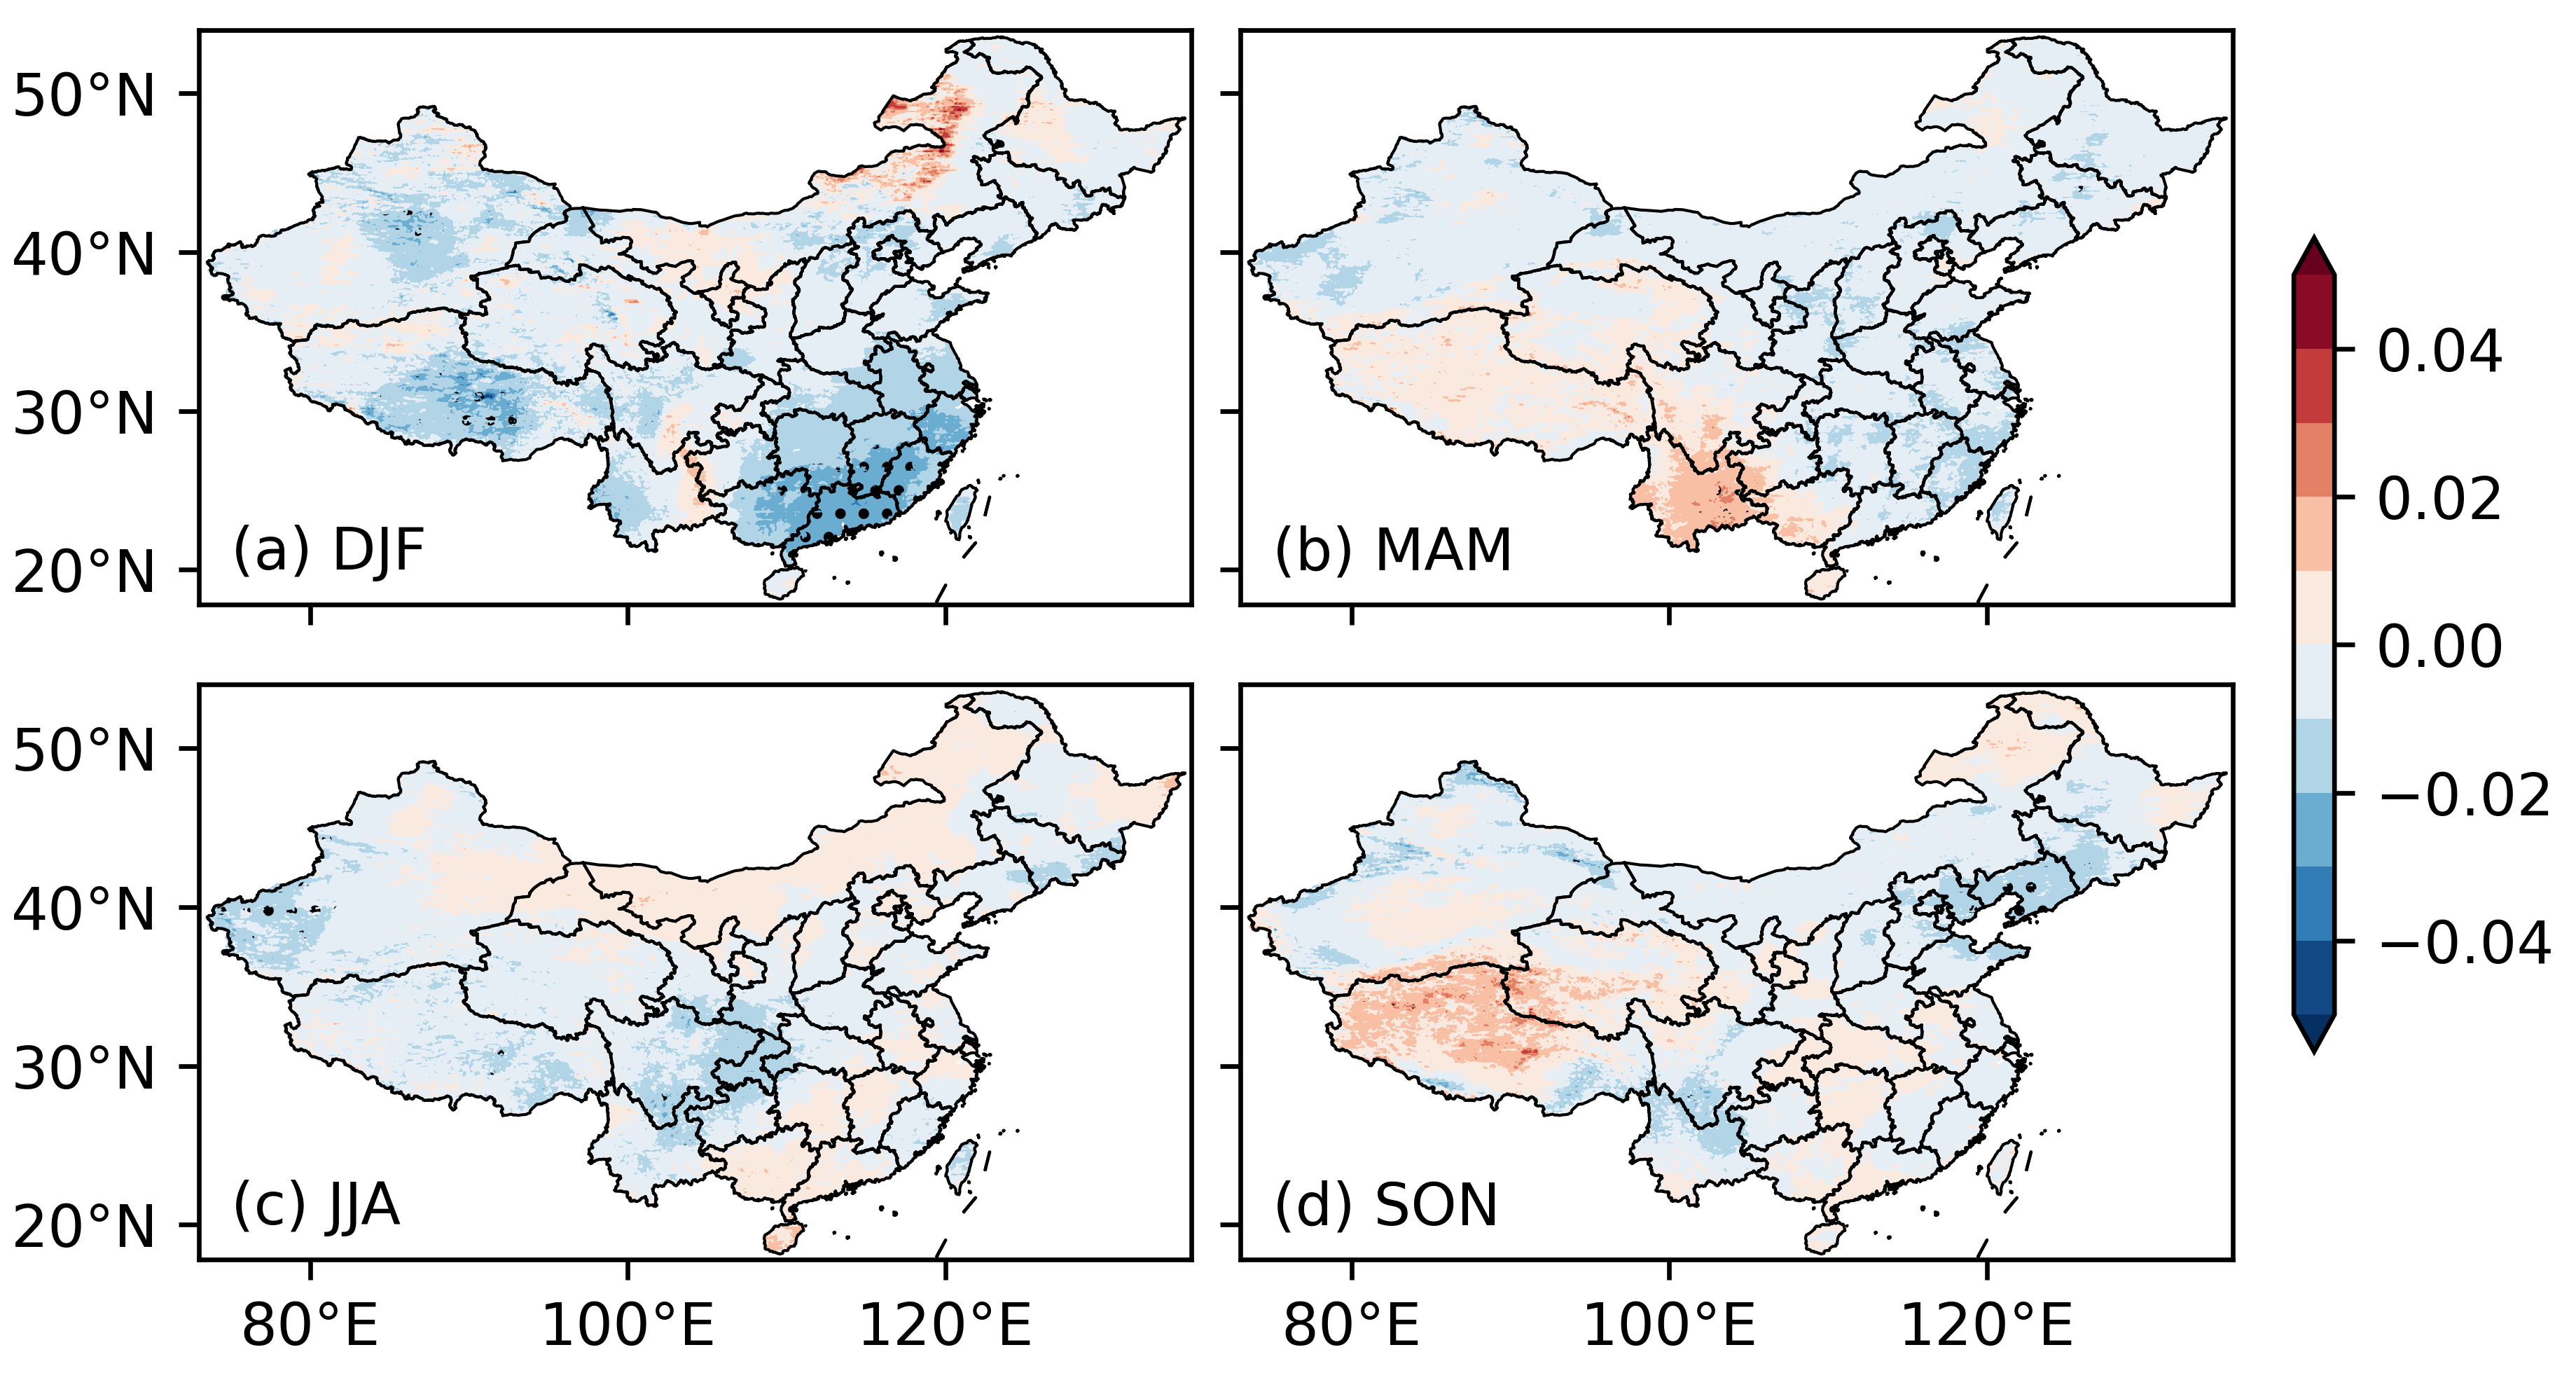
\includegraphics[width=14cm]{fig/anom_elnino.png}
  \caption{Averaged seasonal anomalies in the clearness index during the El~Niño events. Black dots denote the areas with a significance level of 0.1. The four panels (\textbf{a}--\textbf{d}) present winter (DJF), spring (MAM), summer (JJA), and autumn (SON), respectively.\label{fig:elnino}}
\end{figure}

Figure~\ref{fig:lanina} is the same as Figure~\ref{fig:elnino} but averaged over all the La~Niña events. In contrast with the El~Niño events, the La~Niña events increase the clearness index in most areas of China. This increase would be the result of an enhanced northeasterly wind anomaly during the La~Niña events~\cite{sun2018JGRA}. In spring, autumn, and winter, the anomaly patterns are the reverse of the El~Niño events. Compared to the El~Niño events (Figure~\ref{fig:elnino}d), the anomaly magnitude for the La~Niña events is larger, especially in autumn and eastern Yunnan and northeast China (Figure~\ref{fig:lanina}d). It is also interesting to note that the summertime anomaly (Figure~\ref{fig:lanina}c) is not the reverse of the El~Niño events (Figure~\ref{fig:elnino}c), except in southwest China. The anomalies in southwest China may be due to the variations in the Indian monsoon. In other areas, we hypothesize that the clearness index is a result of competing impacts from the Indian monsoon and the East Asian monsoon~\cite{wang2012JGRA}; this hypothesis needs further investigation.

\begin{figure}[H]
    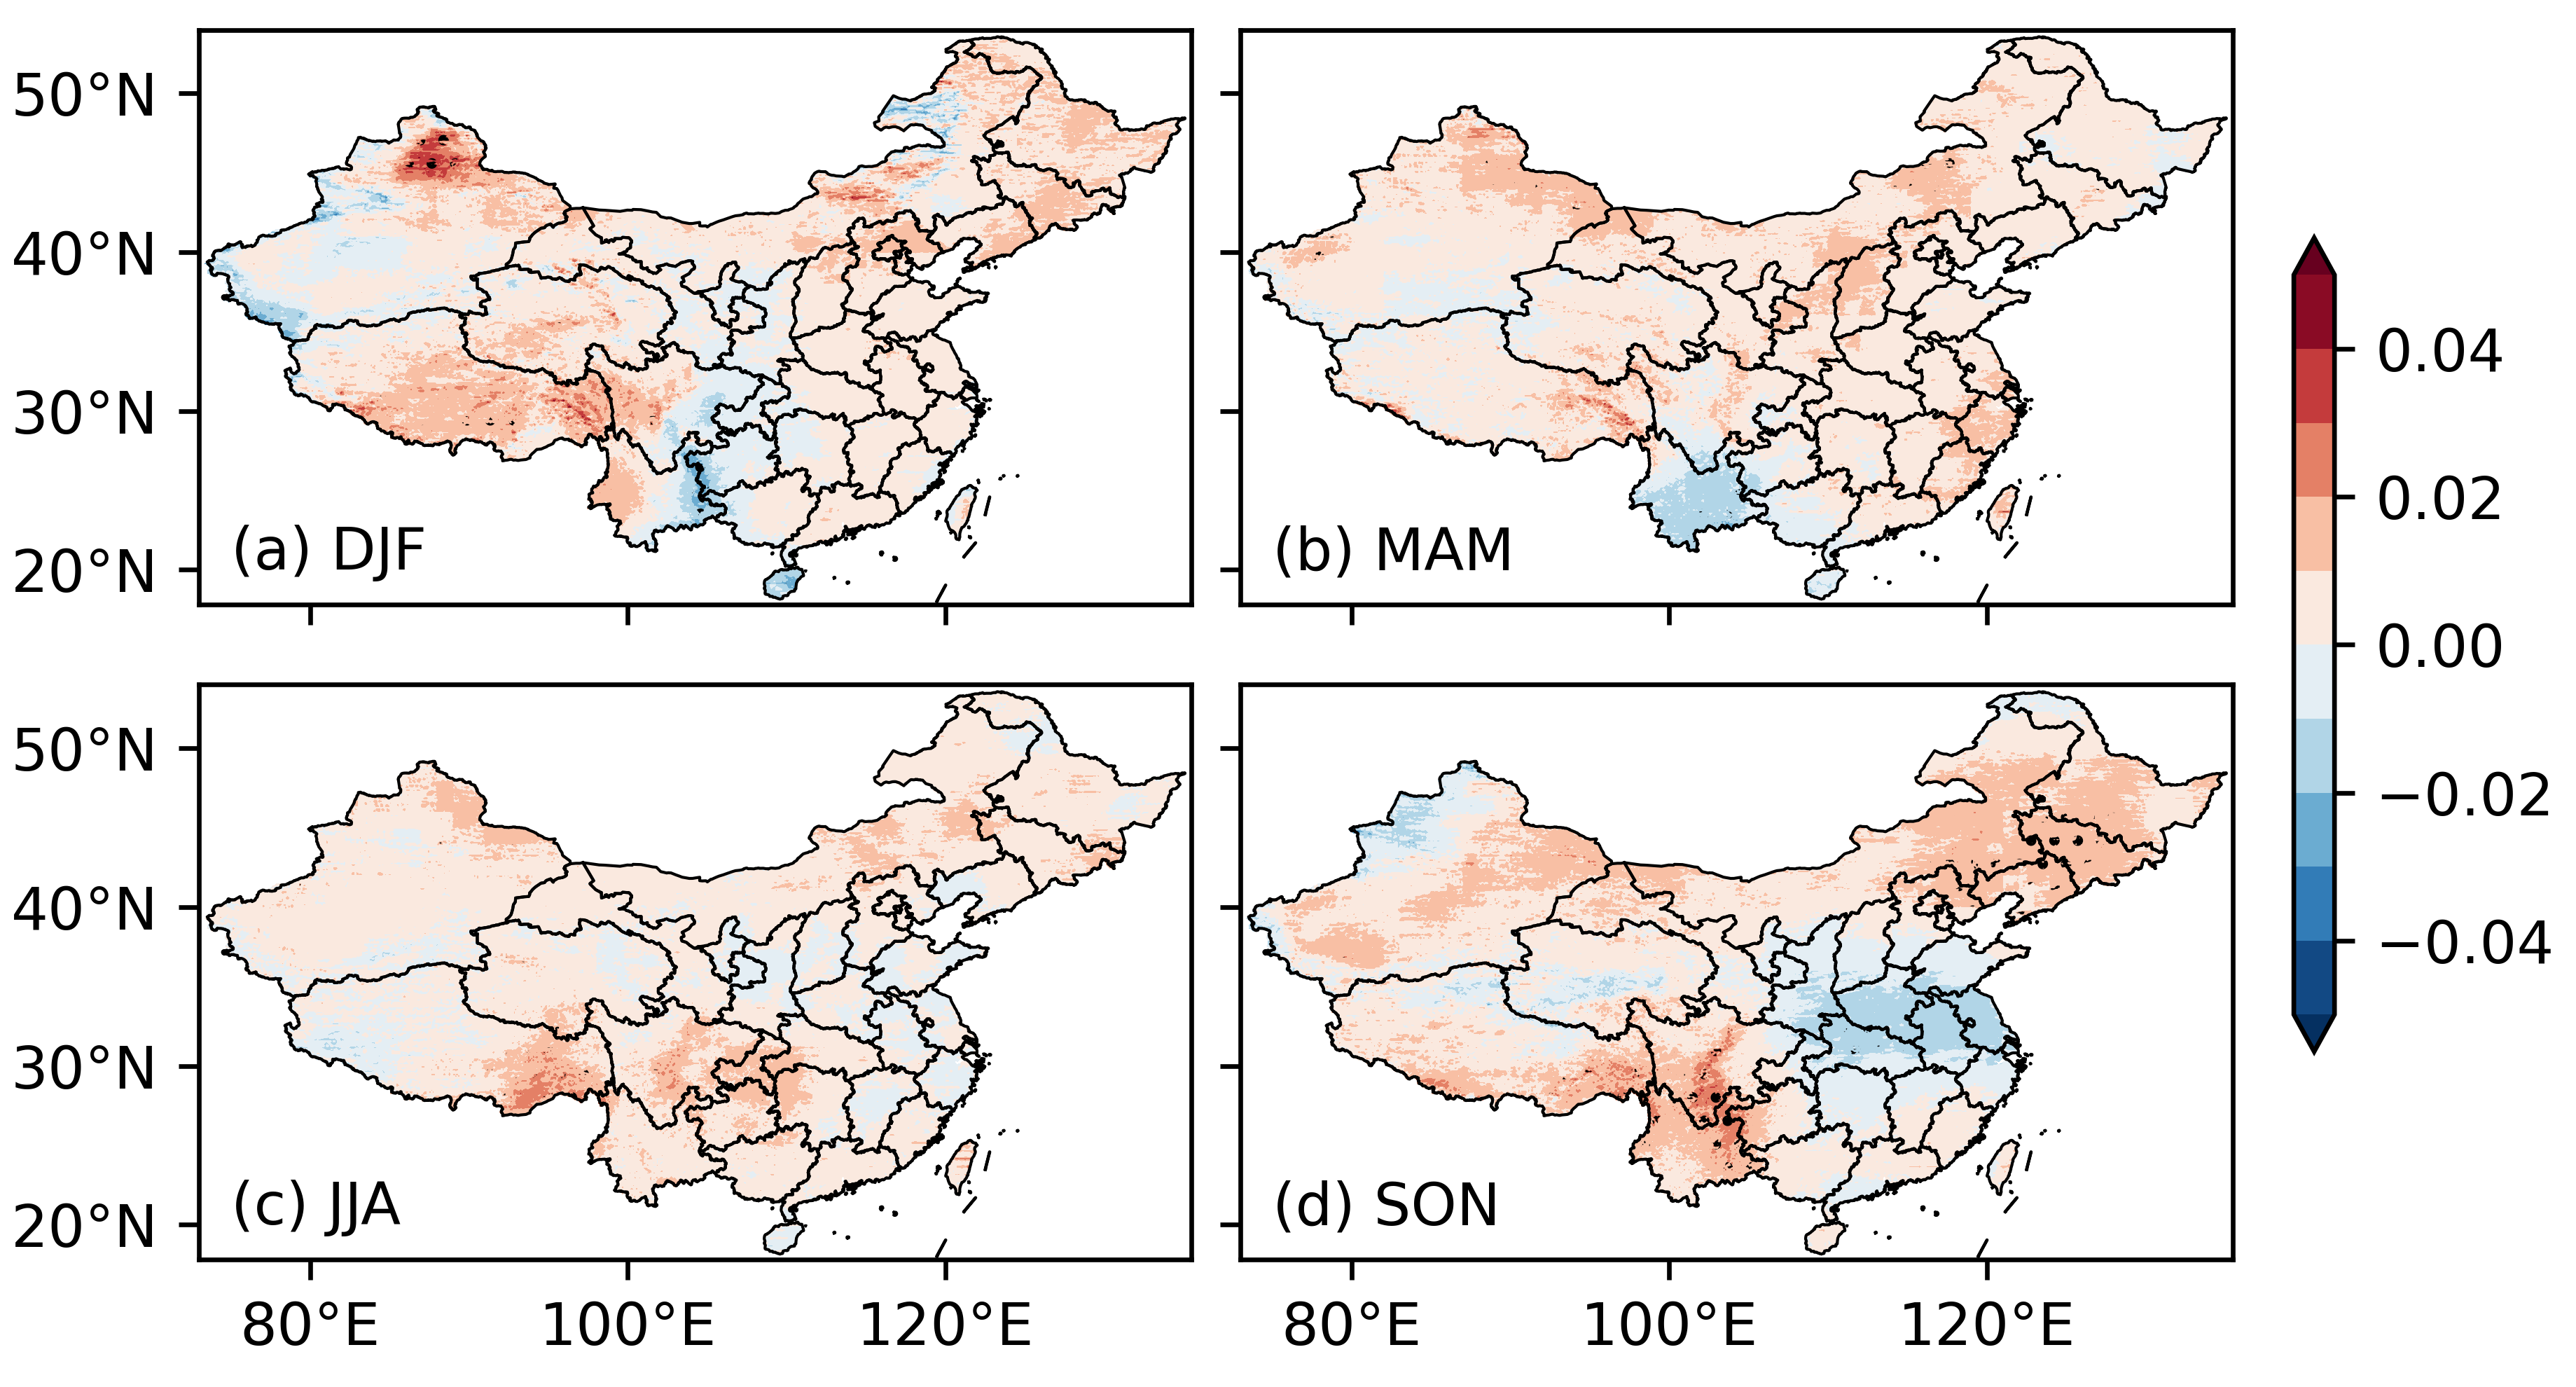
\includegraphics[width=14cm]{fig/anom_lanina.png}
  \caption{Same as Figure~\ref{fig:elnino}, but for La~Niña events. \label{fig:lanina}}
\end{figure}

Figures~\ref{fig:strongelnino} and \ref{fig:stronglanina} are the averaged anomalies for the strong El~Niño and La~Niña events, respectively. In winter, spring, and autumn, for both types of ENSO events, the anomalies scale up with the strength of the events: the magnitude is amplified for the strong events, while the spatial distribution is almost the same. Strong El~Niño events could amplify the influence on the springtime clearness index in the southeastern coastal regions and the autumn clearness index in northeast China. Strong El~Niño can also reduce the springtime clearness index in most northern parts of China. The impacts of strong La~Niña events are the reverse of those of the strong El~Niño events in winter, spring, and autumn. In autumn, strong La~Niña events reduce the clearness index in the middle of eastern China, while increasing the clearness in northeast China. The changes are more significant when compared with strong El~Niño events' impacts.

\begin{figure}[H]
    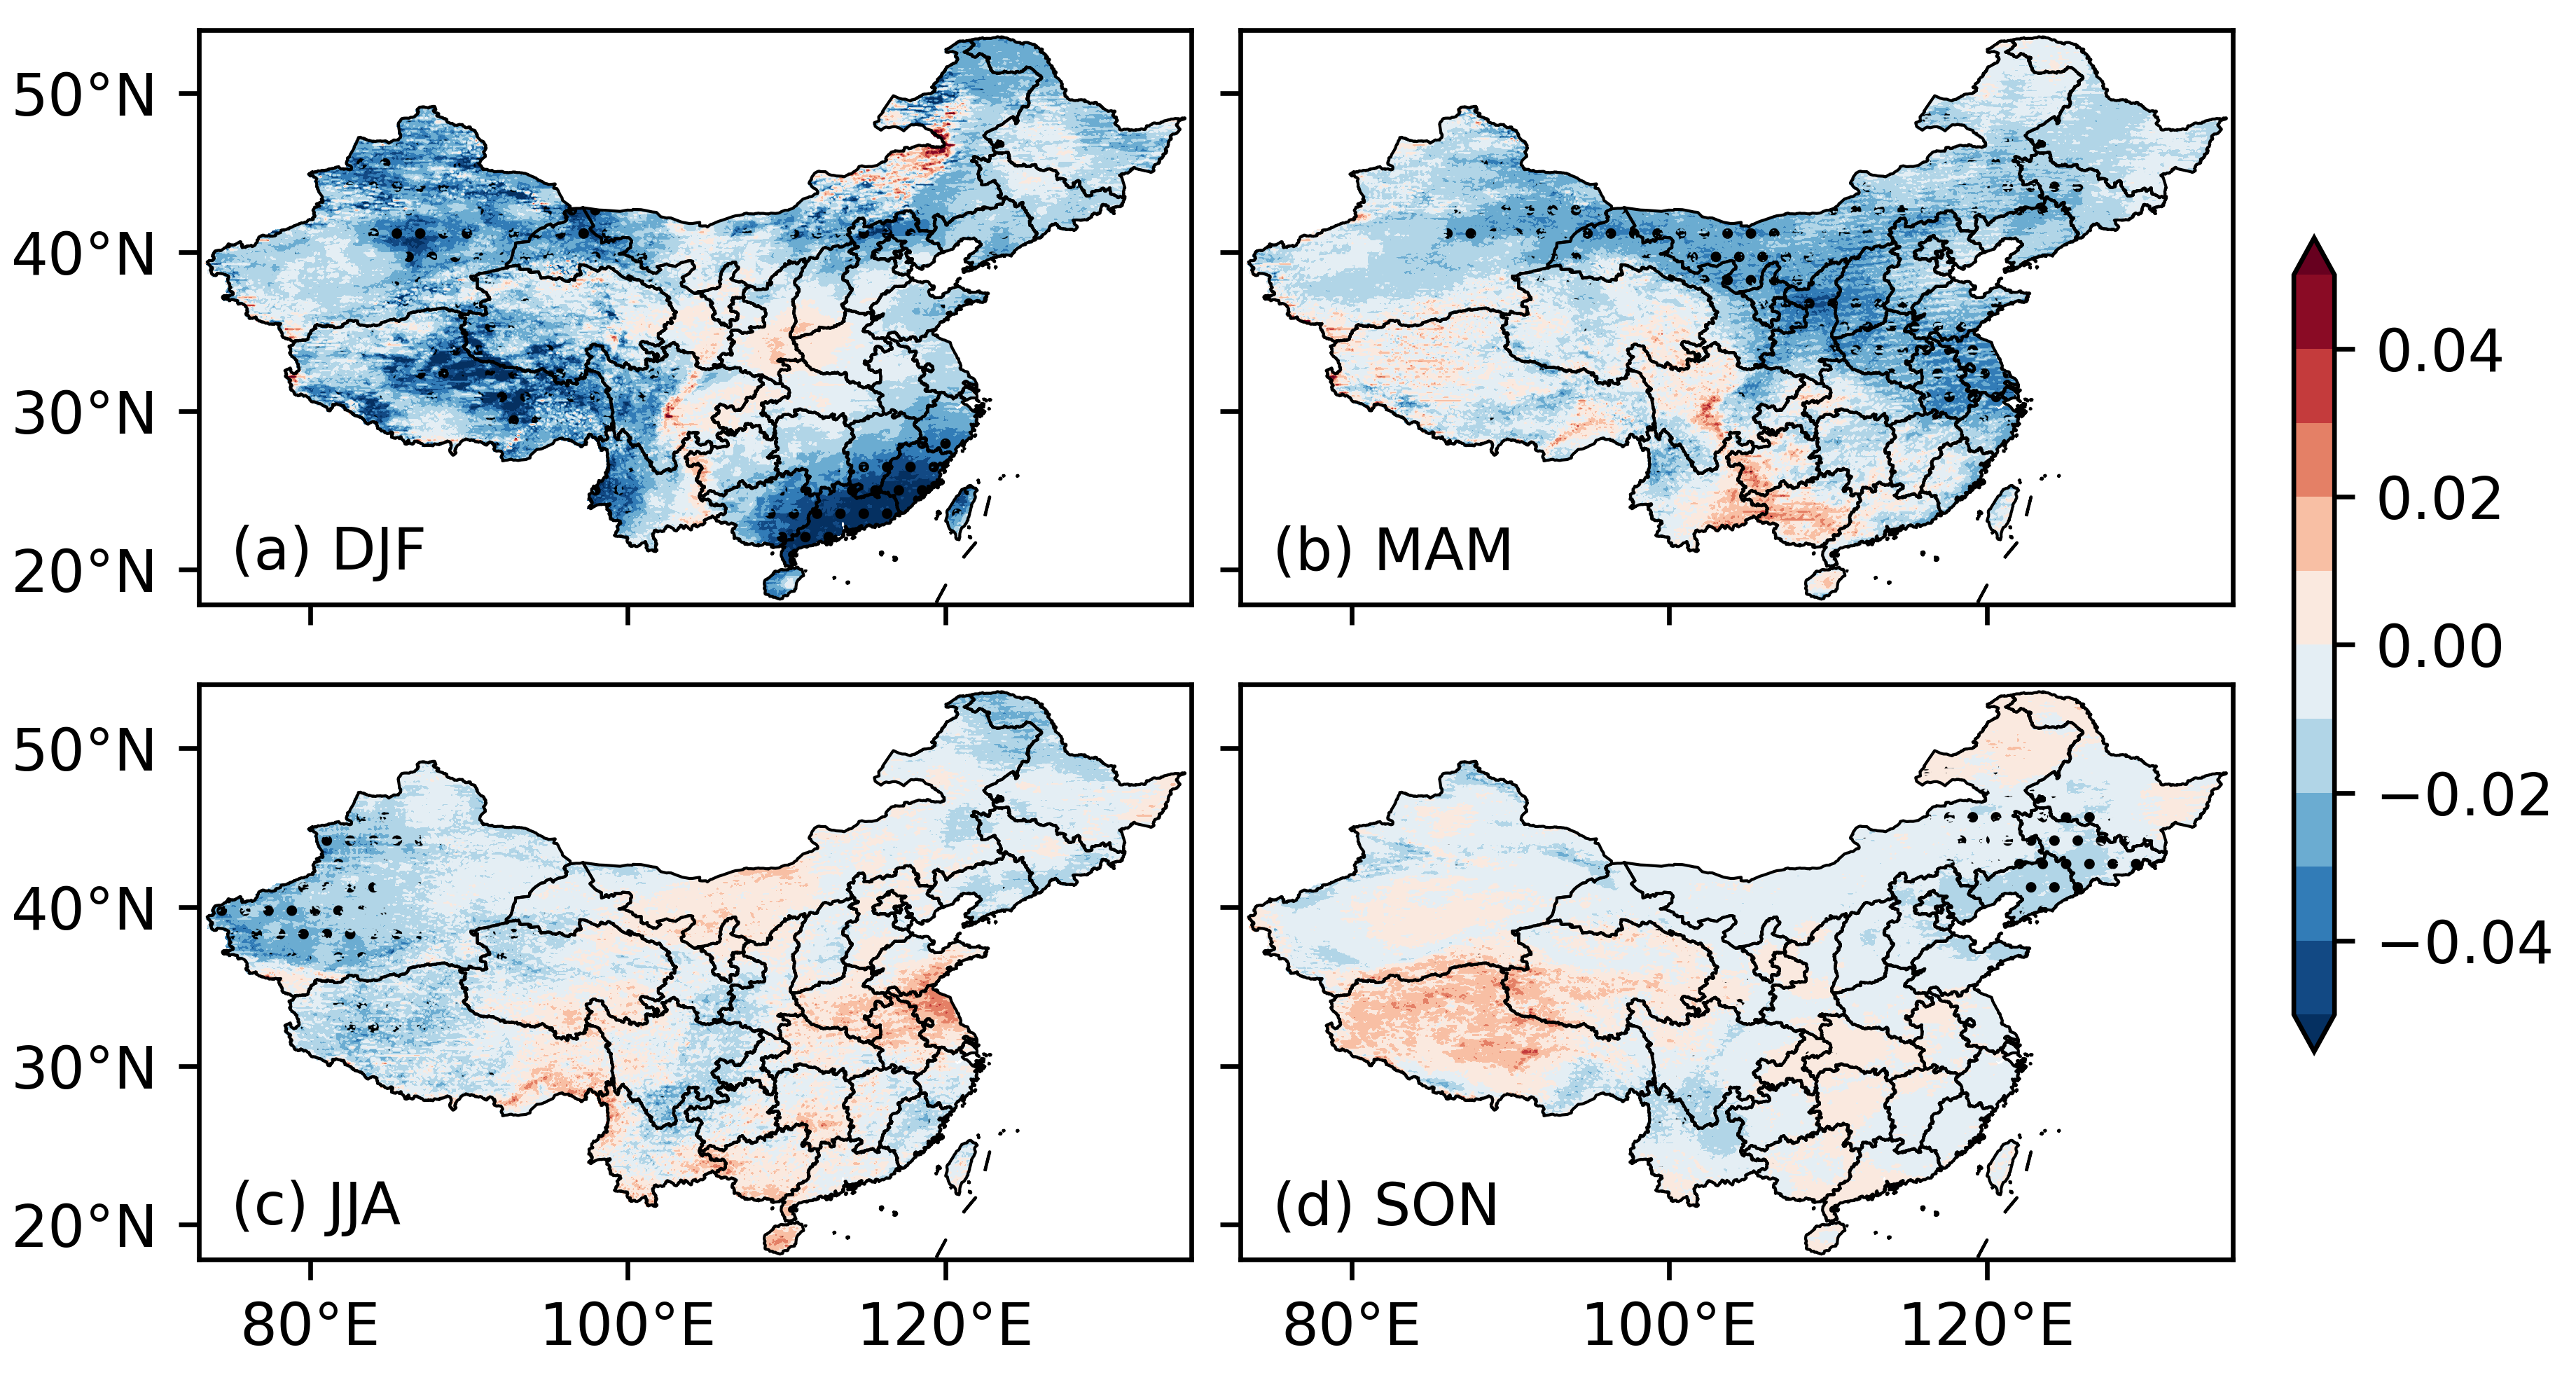
\includegraphics[width=14cm]{fig/anom_strongelnino.png}
  \caption{Same as Figure~\ref{fig:elnino}, but for strong El~Niño events. \label{fig:strongelnino}}
\end{figure}

In the summer following the strong events, the anomalies (Figures~\ref{fig:strongelnino}c and \ref{fig:stronglanina}c) are not simply an amplification of the anomalies in the moderate events (Figures~\ref{fig:elnino}c and \ref{fig:lanina}c). During strong La~Niña events, the summertime anomaly exhibits a reversed tripolar pattern, with an increase in south and north China and a decrease in between. The difference in the spatial patterns between Figures~\ref{fig:stronglanina}c and \ref{fig:lanina}c suggests that the impacts of the La~Niña events are dependent on the strength of the events, which is consistent with previous studies on aerosol concentration~\cite{feng2017JGRA}. The clearness index covariates with precipitation~\cite{huang1989AAS, huang2012AAS}. The covariance rather than negative covariance hints that the relationship between the clearness index and precipitation (i.e., the higher the precipitation, the lower the clearness index) may change with the strength of the La~Niña events, which needs further investigation. For strong El~Niño events, the anomalies are still not significant in most areas of eastern China.


\begin{figure}[H]
    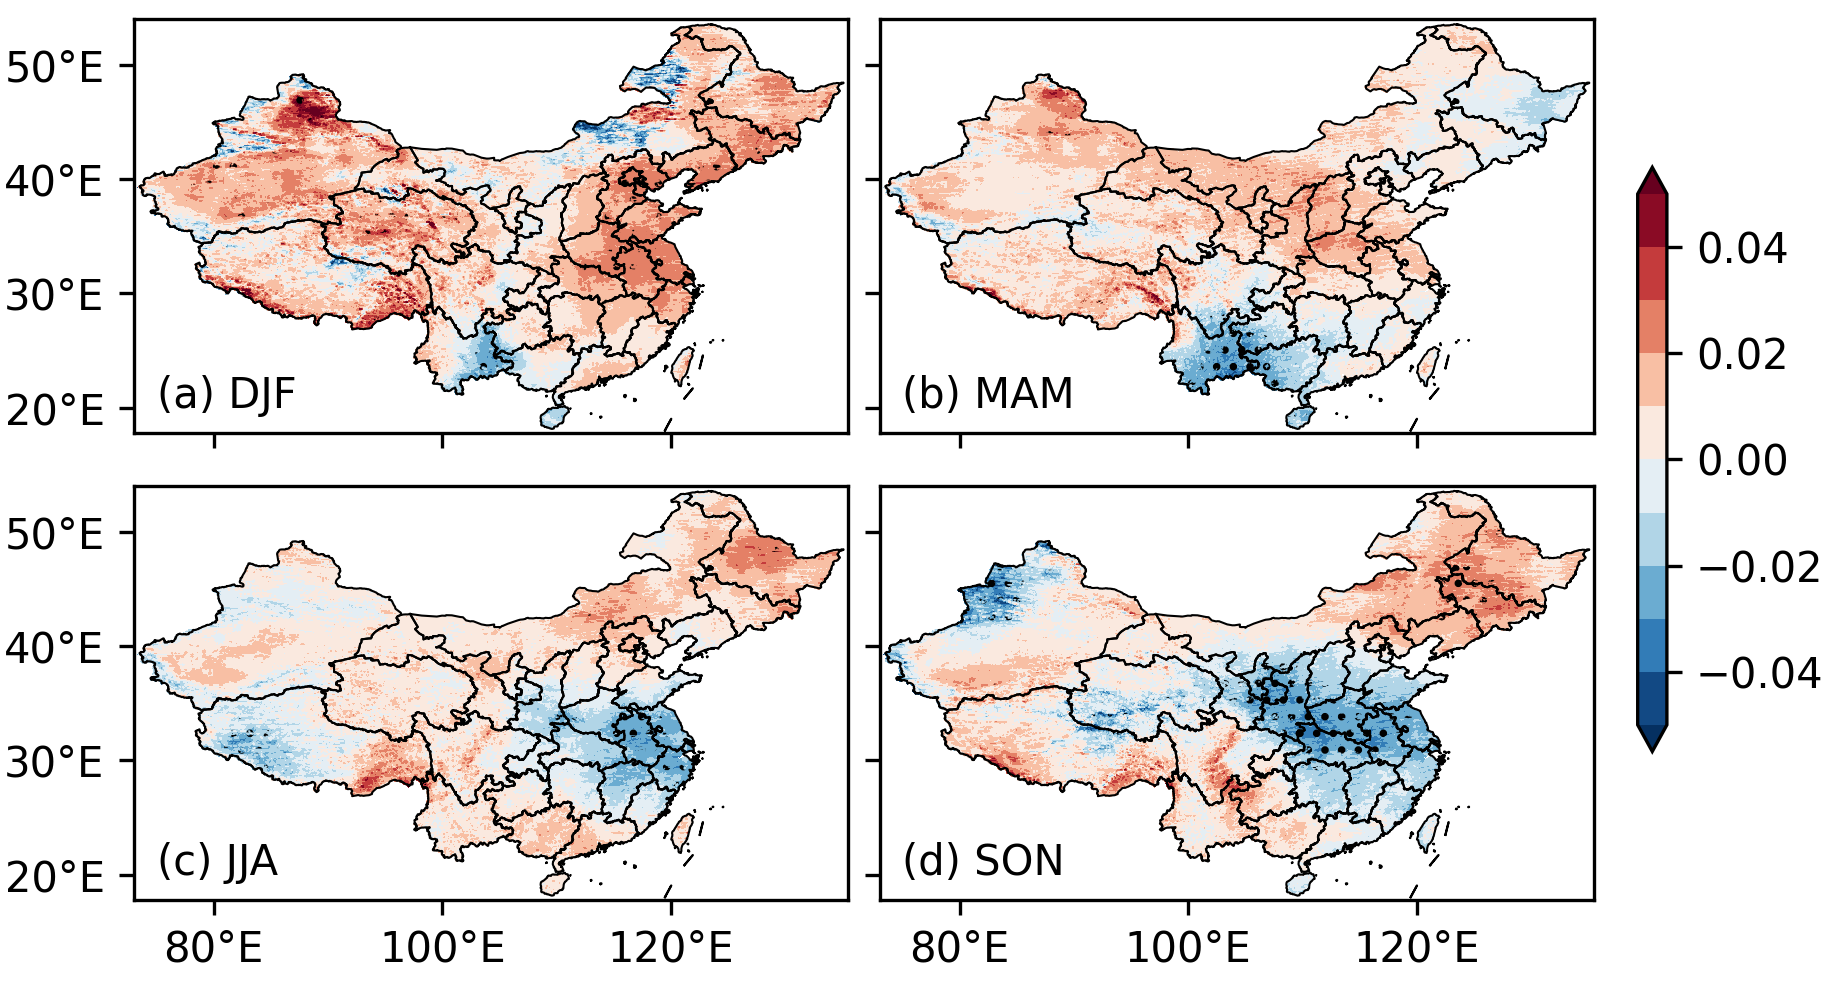
\includegraphics[width=14cm]{fig/anom_stronglanina.png}
  \caption{Same as Figure~\ref{fig:lanina}, but for strong La~Niña events. \label{fig:stronglanina}}
\end{figure}

% %%
\section{Conclusions}\label{sec:conclusions}

We have derived the clearness index as the ratio of global horizontal solar radiation to extraterrestrial radiation. The global horizontal solar radiation is obtained from the CMFD v1.7, and the extraterrestrial radiation is calculated using astronomical geometry. The spatial distributions and seasonal and interannual variations of the clearness index are delineated. The correlation between the interannual anomaly and the Niño-3.4 index is analyzed. The impacts of the El~Niño and La~Niña events of different strengths on the clearness index are revealed.

The nationally averaged clearness index is 0.51. The clearness index is higher in the northern and western regions and lowest in the border areas among Sichuan, Chongqing, and Guizhou. The clearness index has significant seasonal variability in the southern Tibetan Plateau, northeast China, and eastern Sichuan Basin. The interannual variability has a similar spatial distribution, whereas the magnitude is smaller. Among the four seasons, the interannual variability in winter is the largest.

The correlation between the clearness index and the Niño-3.4 index is statistically significant in the southeastern coastal regions of China, northeastern Xizang, and northern Xinjiang, and the areas from northern Hebei to middle Inner Mongolia. The variations in the clearness index in these areas are linked to the ENSO-induced anomalies in the western Pacific subtropical high, the Indian monsoon, the northeast China low, and the South Asia high, respectively.

The impacts of El~Niño and La~Niña events on the clearness index are seasonally dependent. In winter, spring, and autumn, the anomalies in the clearness index are opposite between the El~Niño and La~Niña events. The El~Niño events tend to decrease the clearness index in most areas of China, whereas the La~Niña events tend to increase the clearness index. The significant negative impacts of El~Niño occur in the southeastern coastal regions of China in winter and the areas around Beijing in autumn. The significant positive impacts of La~Niña occur in most areas of eastern China in winter, the middle of eastern China in spring, and northeast China in autumn. The anomalies in strong events are generally amplified in magnitude but are almost invariant with the spatial distribution.

Summer exhibits different anomaly patterns from the other seasons, and the anomalies in the clearness index vary with the strength of the events, especially for La~Niña. Averaged across all the La~Niña events, there is a positive anomaly broadly across China. During strong La~Niña events, the anomaly in the clearness index shows a tripolar pattern in summer, with an increase in South and North China and a decrease in between. The clearness index covariates with the precipitation here: the higher the precipitation, the higher the clearness index. The covariance rather than the commonly found negative covariance hints that the relationship between the clearness index and precipitation may change with the strength of the La~Niña events.

This study provides valuable insights into the interannual variations of atmosphere clearness in China. The findings highlight the nonlinear and multifaceted impacts of ENSO on the clearness index. Further investigation of the atmospheric dynamics and human alternation is necessary for a full understanding of the clearness variation, which is important for solar energy development. The findings of this study would serve as clues for these investigations.

% %%
\vspace{6pt}

% %%
\authorcontributions{Conceptualization, H.Z.; methodology, H.Z.; data curation, H.Z.; investigation, Z.S.; formal analysis, Z.S.; visualization, Z.S.; supervision, H.Z.; project administration, Z.S.; funding acquisition, Z.S.; All authors have contributed to the writing and agreed to the published version of the manuscript. All author have read and agreed to the published version of the manuscript.}

\funding{This research was funded by the Science and Technology Project ``The Research of Mechanism and Simulation on the Interaction between the Local Climate and Large-scale Renewable Energy Development'' (Grant No.\ 4000-202155465A-0-0-00) of State Grid Corporation of China (SGCC).}

\institutionalreview{Not applicable}

\informedconsent{Not applicable}

\dataavailability{The Niño-3.4 index and Oceanic Niño Index were downloaded from the NOAA website (\url{https://psl.noaa.gov/data/climateindices/list/} accessed on 30 December 2023. The CMFD version 1.7 was provided by Jie He at the Institute of Tibetan Plateau Research, Chinese Academy of Sciences. Earlier versions of CMFD are downloadable at \url{https://doi.org/10.11888/AtmosphericPhysics.tpe.249369.file} accessed on 14 November 2023. The data and plotting scripts used in this paper are available at \url{https://gitlab.com/zhenghui88/paper-enso-china-clearness-iav}.}

\acknowledgments{We sincerely thank Jie He at the Institute of Tibetan Plateau Research for his kindness in providing the latest version of CMFD\@.}

\conflictsofinterest{The authors declare no conflicts of interest.}

% %%
\begin{adjustwidth}{-\extralength}{0cm}
  %\printendnotes[custom] % Un-comment to print a list of endnotes

  \reftitle{References}

  \bibliography{references.bib}

  \PublishersNote{}
\end{adjustwidth}
\end{document}
